Consider a powergrid with $C$ consumers and $G$ generators. We are interested
in connecting each consumer to a single generator, but each generator has a
limited capacity and the consumer draws a certain amount of power from the
generator. A valid powergrid is built in such a way that all consumers are
serviced by a generator and that no generator is being overdrawn by too many
consumers. Although consumers and generators may be connected through a complex
network, we analyze the simple case where any consumer is able to attach to any
generator.

\begin{wrapfigure}{r}{0.5\textwidth}
   \begin{center}
      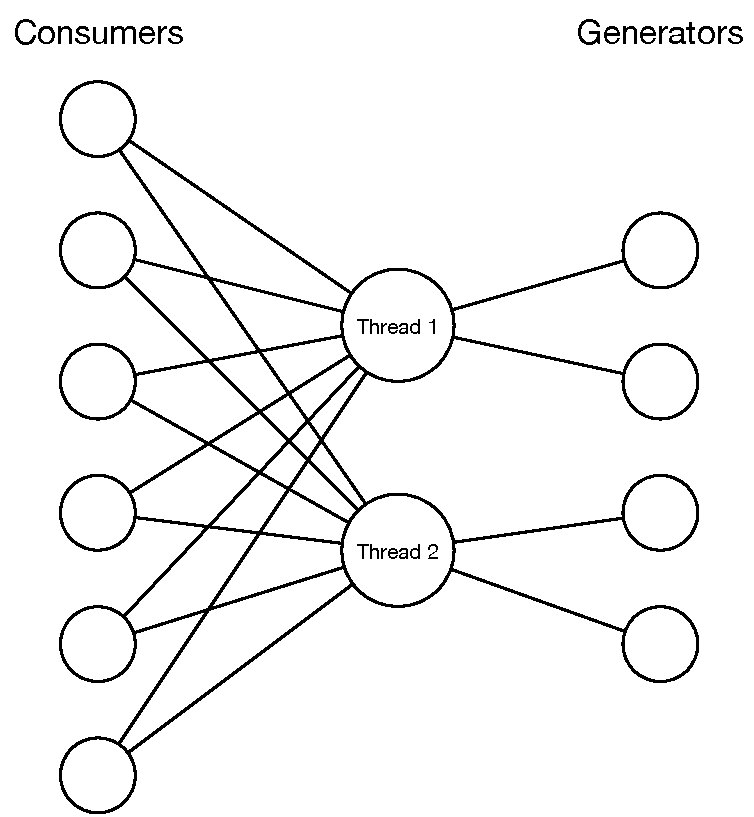
\includegraphics[width=1\linewidth]{figures/threads/powergrid.pdf}
   \end{center}
   \caption{Configuration of a powergrid with 6 consumers, 4
      generators and 2 threads, with each thread responsible for 2 generators.}
   \label{fig:threads:powergrid}
\end{wrapfigure}

A straightforward distributed implementation for the powergrid problem requires
that each consumer is able to connect to a any generator.  Once a generator
receives a connection request, it may or may not accept it.  If the generator
has no power available for the new consumer, it will disconnect from it and the
consumer must select another generator. This randomized algorithm works but can
take a long time time to converge, depending on the amount of power available in
the generators.

\begin{figure}[h!]
\begin{Verbatim}[numbers=left,fontsize=\scriptsize,commandchars=*\#\&]
node generator.
node consumer.
type linear capacity(generator, int Total, int Used).
type linear connected-to(generator, consumer, int).
type linear connected-to-list(generator, list consumer).
type power(consumer, int).
type linear disconnected(consumer).
type linear connected(consumer, generator).
type generators(consumer, list generator).
type linear fails(generator, int).
type linear random-reconnect(generator).
type linear reconnect(consumer).
type linear connect(generator, consumer, int).
type linear disconnect(consumer, generator).

connected-to-list(G, []).  fails(G, 0).
disconnected(C).  reconnect(C).  !generators(C, all-generators).

fails(G, Fails), Fails > maxfails
   -o random-reconnect(G).

capacity(G, Total, Used), random-reconnect(G),
connected-to-list(G, L), L <> [], C = nth(L, randint(length(L))),
connected-to(G, C, Power)
   -o fails(G, 0), capacity(G, Total, Used - Power),
      connected-to-list(G, remove(L, C)),
      disconnect(C, G).

capacity(G, Total, Used), random-reconnect(G)
   -o capacity(G, Total, Used), fails(G, 0).

connect(G, C, Power), capacity(G, Total, Used),
fails(G, Fails), connected-to-list(G, L),
Used + Power <= Total
   -o capacity(G, Total, Used + Power),
      fails(G, max(Fails - 1, 0)), connected-to(G, C, Power),
      connected-to-list(G, [C | L]).

connect(G, C, Power), capacity(G, Total, Used),
Used + Power > Total, fails(G, Fails)
   -o capacity(G, Total, Used), disconnect(C, G),
      fails(G, Fails + 1).

!generators(C, L), !power(C, Power),
reconnect(C), disconnected(C),
G = nth(L, randint(num-generators))
   -o connected(C, G), connect(G, C, Power).

disconnect(C, G), connected(C, G)
   -o disconnected(C), reconnect(C).
\end{Verbatim}
\caption{LM code for the regular powergrid program.}
\label{code:threads:powergrid}
\end{figure}

The issue with the straightforward distributed implementation is that it lacks a
global view of the problem or requires a more complicated synchronization
algorithm between consumers and generators. As we have seen before, thread local
facts are an excellent mechanism to introduce a global view of the problem
without complicating the original algorithm written in a declarative style.  In
our solution, we partition the set of generators $G$ among the threads in the
system. With this partitioning, each thread assumes the ownership of its
generators and is able to process consumers with a global view over its set of
generators. The thread can then immediately assign the consumers to its
generators when possible. Figure~\ref{fig:threads:powergrid} shows how a powergrid
configuration is re-configured to take into account the number of available
threads. We have implemented both the \code{Regular} and the \code{Optimized}
algorithms in LM.

\begin{figure}[h!]
\begin{Verbatim}[numbers=left,fontsize=\scriptsize,commandchars=*\#\&]
type linear thread-connected-to(thread, generator, consumer, int).
type linear thread-connected-to-list(thread, generator, list consumer).
type linear thread-capacity(thread, generator, int, int).
type linear thread-total-capacity(thread, int, int).
type linear start(generator).

thread-total-capacity(T, 0, 0).
fails(G, 0).  disconnected(C).  reconnect(C).  !generators(C, all-generators).  start(G).

start(G), !generator-id(G, Id)
   -o set-cpu(G, Id % @threads).

just-moved(G), capacity(G, Total, Used), thread-total-capacity(T, TotalCapacity, TotalUsed)
   -o thread-connected-to-list(T, G, []), thread-capacity(T, G, Total, Used),
      thread-total-capacity(T, Total + TotalCapacity, Used + TotalUsed).

fails(G, Fails), Fails > maxfails
   -o random-reconnect(G).

thread-capacity(T, G, Total, Used), thread-total-capacity(T, TotalCapacity, TotalUsed),
random-reconnect(G), thread-connected-to-list(T, G, L), L <> [], C = nth(L, randint(length(L))),
thread-connected-to(T, G, C, Power), NewUsed = Used - Power
   -o fails(G, 0), thread-capacity(T, G, Total, NewUsed),
      thread-total-capacity(T, TotalCapacity, TotalUsed - Power),
      thread-connected-to-list(T, G, remove(L, C)), disconnect(C, G).

random-reconnect(G)
   -o fails(G, 0).

connect(G, C, Power), thread-total-capacity(T, TotalCapacity, TotalUsed),
thread-capacity(T, G, Total, Used), fails(G, Fails), thread-connected-to-list(T, G, L),
NewUsed = Used + Power, NewUsed <= Total
   -o thread-capacity(T, G, Total, NewUsed),
      thread-total-capacity(T, TotalCapacity, TotalUsed + Power),
      fails(G, max(Fails - 1, 0)), thread-connected-to(T, G, C, Power),
      thread-connected-to-list(T, G, [C | L]).

connect(G, C, Power), thread-capacity(T, G, Total, Used), Used + Power > Total, fails(G, Fails)
   -o thread-capacity(T, G, Total, Used), disconnect(C, G), fails(G, Fails + 1).

!power(C, Power), reconnect(C), disconnected(C), thread-total-capacity(T, TotalCapacity, TotalUsed),
TotalNewUsed = TotalUsed + Power, NewUsed <= TotalCapacity,
thread-capacity(T, G, Total, Used), thread-connected-to-list(T, G, ConnectList),
NewUsed = Used + Power, NewUsed <= Total
   -o connected(C, G), thread-capacity(T, G, Total, NewUsed),
      thread-connected-to-list(T, G, [C | ConnectList]), thread-connected-to(T, G, C, Power),
      thread-total-capacity(T, TotalCapacity, TotalNewUsed).

!generators(C, L), !power(C, Power), reconnect(C), disconnected(C), G = nth(L, randint(num-generators))
   -o connected(C, G), connect(G, C, Power).

disconnect(C, G), connected(C, G)
   -o disconnected(C), reconnect(C).
\end{Verbatim}
\caption{LM code for the optimized powergrid program.}
\label{code:threads:powergridt}
\end{figure}

\clearpage
